\qs{}{
    What are the combinations of semester and school year?
}

Retrieve \texttt{DISTINCT} combinations of academic semesters (referred to as \texttt{adm\_sem}) and the corresponding formatted admission years (as \texttt{school\_year}) from the \texttt{admission} table. \texttt{ORDER} the results first by the school year and then by the academic semester, ensuring that the output is sorted in ascending order based on the school year and within the same year by academic semester.
\vspace{\baselineskip}

\sol{}
\noindent\line(1, 0){0.89\linewidth}
\begin{verbatim}
SELECT DISTINCT adm_sem, DATE_FORMAT(adm_year, '%Y') AS school_year
FROM admission
ORDER BY school_year, adm_sem;
\end{verbatim}
\noindent\line(1, 0){\linewidth}

\begin{figure}[H]
    \centering
    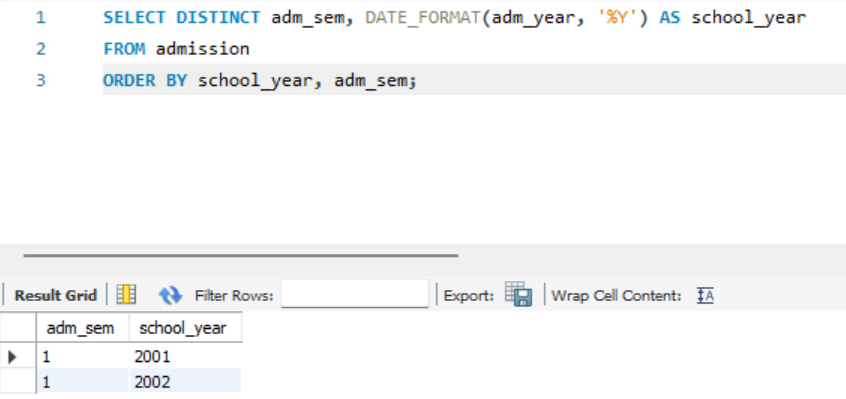
\includegraphics[width=0.7\linewidth]{images/q6.png}
    \caption{Question 6 Query and Output}
\end{figure}
